%% ============================================================
%% 分片 05：原文第 3 节「Topological Field Theory From ${\EUN}=4$ Super Yang-Mills Theory」（原文 glshort.tex 起于第 1216 行）
%% 由 tools/harvmac2tex.py 从 arXiv 源码（hep-th/0604151v3）自动生成。
%% 只译英文散文；公式、编号、\label、\cite 一律不改。
%% ============================================================

\subsection{Twisting ${\EUN}=4$ Super Yang-Mills}

\label{sec:twisting}

\par\medskip{\it General Idea Of Twisting}

  

 ${\EUN}=2$ super Yang-Mills theory can be twisted to make a
quantum field theory realization of Donaldson theory \cite{ref25}.
Similarly \cite{ref45}, ${\EUN}=4$ super Yang-Mills theory can be
twisted in three ways to make a topological field theory.  Two of
the twisted theories, including one that was investigated in
detail in \cite{ref45}, are closely analogous to Donaldson theory
in the sense that they lead to instanton invariants which, like
the Donaldson invariants of four-manifolds, can be expressed in
terms of the Seiberg-Witten invariants.   The third twist, which
was mentioned in \cite{ref52}\ and has been investigated in
\cite{ref53,ref54,ref55,ref56,ref57}, has had no applications until now. It
turns out to be the twist relevant to the geometric Langlands
program, and we will call it the GL twist.

To give an inevitably very brief explanation of the notion of
twisting, we first take $M=\Bbb{R}^4$. This has rotational
symmetry group $Spin(4)$, of course, while the ${\EUN}=4$ theory
has the larger symmetry $Spin(4)\times Spin(6)$.
 ``Twisting'' means replacing
$Spin(4)$ by a different subgroup $Spin'(4)$ of $Spin(4)\times
Spin(6)$ that is isomorphic to $Spin(4)$ and acts on $\Bbb{R}^4$
the same way that $ Spin(4)$ does, but acts differently on the
${\EUN}=4$ gauge theory. To accomplish this, we pick a
homomorphism $\varkappa:Spin(4)\to Spin(6)$ and set
$Spin'(4)=(1\times \varkappa)(Spin(4))\subset Spin(4)\times
Spin(6)$.

We also want to pick $\varkappa $ such that the action of
$Spin'(4)$ on ${\EUS}^+$ has a non-zero invariant vector.  Since
the supersymmetry generator $\epsilon$ takes values in  $
{\EUS}^+$, a choice of  an invariant vector in ${\EUS}^+$ will
give us a $Spin'(4)$-invariant supersymmetry that we will call
$Q$.  It will automatically obey $Q^2=0$, by virtue of \eqref{eq:ugo}.
(There is no $Spin'(4)$ invariant operator on the right hand side
of \eqref{eq:ugo}, so as $Q^2=\half\{Q,Q\}$ is $Spin'(4)$-invariant, it must
vanish.) Once $Q$ is chosen, we change the physical interpretation
of the theory to say that we are only interested in $Q$-invariant
path integrals, operators, and states, and that we consider
anything of the form $[Q,{\EUO}\}$, for any operator ${\EUO}$, to
be trivial. So henceforth, the interesting operators or states lie
in suitable cohomology groups of $Q$.

It turns out that theories obtained this way are, loosely
speaking, topological field theories. (They may depend on the
smooth structure of $M$, which goes into the definition of the
quantum field theory, before or after twisting.) This is proved by
showing that the definition of the theory on flat $\Bbb{R}^4$ can
be extended to any four-manifold in such a way that the $Q$
symmetry is retained and the choice of metric is irrelevant modulo
$Q$-exact terms.
 For the GL twist of ${\EUN}=4$ super Yang-Mills theory,
 one approach to this can be found in section 7 of \cite{ref56}. In
the present paper, we will take another route; once we have worked
out the topological equations and the vanishing theorems, we will
see directly, in section 第~\ref{sec:toplag}~节, what action on a curved
four-manifold has the right properties.

\par\medskip{\it Description Of Twist}

Now we will describe the GL twist. The homomorphism
$\varkappa:Spin(4)\to Spin(6)$ is chosen so that the ${\bf 4}$ of
$Spin(6)=SU(4)_{{\cal R}}$ transforms as $({\bf 2},\bone)\oplus
(\bone,{\bf  2})$ of $Spin(4)=SU(2)\times SU(2)$, which we will
refer to as $SU(2)_\ell\times SU(2)_\rr$.\footnote{ The ``$\ell$'' and
``$r$'' in $SU(2)_\ell$ and $SU(2)_\rr$ are usually read as
``left'' and ``right,'' referring to the spin of physical massless
particles.} (The $\bar{\bf 4}$ of $Spin(6)$, which is the complex
conjugate of the ${\bf 4}$, transforms the same way under
$Spin(4)$, since the $({\bf 2},\bone)$ and $(\bone,{\bf 2})$ of
$Spin(4)$ are pseudoreal.)

This choice of $\varkappa$ amounts to embedding $SU(2)_\ell\times
SU(2)_\rr$ in $Spin(6)=SU(4)_{{\cal R}}$ in the following way:
% 式 (3.2)
\setcounter{equation}{1}
\begin{equation}\label{eq:norml}
\left(\begin{matrix}SU(2)_\ell &  0 \\
                                                  0    &
                                                  SU(2)_\rr\\\end{matrix}\right).
\end{equation}

This embedding obviously commutes with an additional $U(1)$
group,\footnote{The global structure of the combined  group is
actually not a product $SU(2)_\ell\times SU(2)_\rr\times U(1)$,
but rather the quotient $(SU(2)_\ell\times SU(2)_\rr\times
U(1))/\Bbb{Z}_2$.} whose generator ${\cal K}$ we can take to have
the form % 式 (3.3)
\setcounter{equation}{2}
\begin{equation}\label{eq:orml}
{\cal K}=i\left(\begin{matrix}1&  0 \\
                                                  0    &
                                                  -1\\\end{matrix}\right)
\end{equation}

in $2\times 2$ blocks.  So our embedding is such that the ${\bf
4}$ of $Spin(6)$ transforms under $SU(2)_\ell\times
SU(2)_\rr\times U(1)$ as $({\bf 2},\bone)^{1}\oplus (\bone,{\bf
2})^{-1}$, where now the exponent is the eigenvalue of $-i{\cal
K}$, which we will call ${\EUK}$. The $\bar{\bf 4}$ transforms as
the complex conjugate of this, or $({\bf 2},\bone)^{-1}\oplus
(\bone,{\bf 2})^{1}$.

This twist can also be conveniently described in terms of $SO$
groups rather than $Spin$ groups.  To do so, we use the fact that
the fundamental, six-dimensional vector representation ${\bf 6_v}$
of $SO(6)$ is, in terms of $Spin(6)=SU(4)_{{\cal R}}$, the same as
$\wedge^2 {\bf 4}$, the skew-symmetric part of ${\bf 4}\otimes{\bf
4}$. So ${\bf 6_v}=\wedge^2(({\bf 2},\bone)^{1}\oplus (\bone,{\bf
2})^{-1})=(\btwo,\btwo)^0\oplus (\bone,\bone)^2\oplus
(\bone,\bone)^{-2}$.  Here $(\btwo,\btwo)$ is the same as the
vector representation ${\bf 4_v}$ of $SO(4)$. So the ${\bf 6_v}$
is the sum of a vector ${\bf 4_v}$ of $SO(4)$ with ${\EUK}=0$, and
two $SO(4)$  scalars with ${\EUK}=\pm 2$. This corresponds to the
obvious homomorphism of $SO(4)\times U(1)=SO(4)\times SO(2)$ to
$SO(6)$:\footnote{The $U(1)$ in $(SU(2)\times SU(2)\times
U(1))/\Bbb{Z}_2\subset SU(4)$ is a double cover of the $U(1)$ in
$SO(4)\times U(1)\subset SO(6)$.} % 式 (3.4)
\setcounter{equation}{3}
\begin{equation}\label{eq:tomo}
\left(\begin{matrix}SO(4) &
0 \\ 0 & SO(2)\\\end{matrix}\right).
\end{equation}

The six spin zero fields $\phi_i$, $i=0,\dots,5$ of ${\EUN}=4$
super Yang-Mills theory transform as ${\bf 6_v}$ of $SO(6)$, so
this analysis applies to them.  We can pick coordinates so the
first four fields $\phi_0,\dots,\phi_3$ form a ${\bf 4_v}$ of
$SO(4)$, while $\phi_4$ and $\phi_5$ are the $SO(4)$ scalars,
which are rotated by $SO(2)$.  Moreover, we can label the scalars
so that the linear combinations $\sigma=(\phi_4-i\phi_5)/\sqrt 2$
and $\bar\sigma=(\phi_4+i\phi_5)/\sqrt 2$ have ${\EUK}=2$ and
${\EUK}=-2$. The fields $\phi_0,\dots,\phi_3$ can then be
interpreted geometrically as the components of an adjoint-valued
one-form, while $\sigma$ is a scalar field or zero-form with
values in the complexification of the Lie algebra.  So the bosonic
fields of the theory are a gauge field, which locally is an
adjoint-valued one-form $A=A_\mu \,dx^\mu$, along with a second
adjoint-valued one-form $\phi=\phi_\mu\,dx^\mu$, and the complex
scalars $\sigma$ and $\bar\sigma$.

\par\medskip{\it Transformation Of The Supersymmetries}

We can likewise analyze how the supersymmetries transform under
$Spin'(4)$. The $\bar{\bf 4}$ of $Spin(6)$ transforms as
$(\btwo,\bone)^{-1}\oplus (\bone,\btwo)^{1}$ of $Spin'(4)\times
U(1)$, and the ${\bf  4}$ as $(\btwo,\bone)^{1}\oplus
(\bone,\btwo)^{-1}$. So, using \eqref{eq:jugo}, the supersymmetries that
transform as $(\btwo,\bone)$ of $Spin(4)$ transform under
$Spin'(4)\times U(1)$ as % 式 (3.5)
\setcounter{equation}{4}
\begin{equation}\label{eq:lollypop}
(\btwo,\bone)^0\otimes
((\btwo,\bone)^{-1}\oplus (\bone,\btwo)^{1}) =
(\bone,\bone)^{-1}\oplus ({\bf 3},\bone)^{-1}
\oplus(\btwo,\btwo)^{1}.
\end{equation}
 And the supersymmetries that transform
as $(\bone,\btwo)$ of $Spin(4)$ transform under $Spin'(4)\times
U(1)$ as % 式 (3.6)
\setcounter{equation}{5}
\begin{equation}\label{eq:tollypop}
(\bone,\btwo)^0\otimes
((\btwo,\bone)^{1}\oplus (\bone,\btwo)^{-1}) = (\bone,\bone)^{-1}
\oplus (\bone,{\bf 3})^{-1} \oplus(\btwo,\btwo)^{1}.
\end{equation}

Next, we can find the $Spin'(4)$-invariant supersymmetries. {}From
\eqref{eq:lollypop}\ and \eqref{eq:tollypop}, there is one invariant supersymmetry
generator $\epsilon_\ell$ that is left-handed in the
four-dimensional sense (transforms as $({\bf 2},\bone)$ under the
original $Spin(4)$), and one such generator $\epsilon_\rr$ that is
right-handed (transforms as $(\bone,{\bf 2})$). With our
conventions, they are distinguished by
% 式 (3.7)
\setcounter{equation}{6}
\begin{equation}\label{eq:onog}
\begin{aligned}\hat\Gamma_E\epsilon_\ell& = -\epsilon_\ell\\
\hat\Gamma_E\epsilon_\rr& = \epsilon_\rr.\\\end{aligned}
\end{equation}
 A choice of
$\epsilon_\ell$ determines a natural choice of $\epsilon_\rr$,
namely % 式 (3.8)
\setcounter{equation}{7}
\begin{equation}\label{eq:huy}
\epsilon_\rr=N\epsilon_\ell,
\end{equation}
 where $N={1\over
4}\sum_{\mu=0}^3\Gamma_{\mu+4}\Gamma_{\mu}$. This idea here is
that $N$ commutes with $Spin'(4)$ but anticommutes with
$\hat\Gamma_E$, so the definition \eqref{eq:huy}\ makes sense.  We have
normalized $N$ so that $N^2\epsilon=-\epsilon$ if $\epsilon$ is
$Spin'(4)$-invariant. Hence we have also
% 式 (3.9)
\setcounter{equation}{8}
\begin{equation}\label{eq:uy}
\epsilon_\ell=-N\epsilon_\rr.
\end{equation}
 By exploiting the
$Spin'(4)$ symmetry, one can show that for $\mu=0,\dots,3$, we
have % 式 (3.10)
\setcounter{equation}{9}
\begin{equation}\label{eq:uzu}
\Gamma_{\mu+4}\epsilon_\ell =
-\Gamma_\mu\epsilon_r,~\Gamma_{\mu+4}\epsilon_r=\Gamma_\mu\epsilon_\ell.
\end{equation}

\begin{figure}[htbp]
\centering
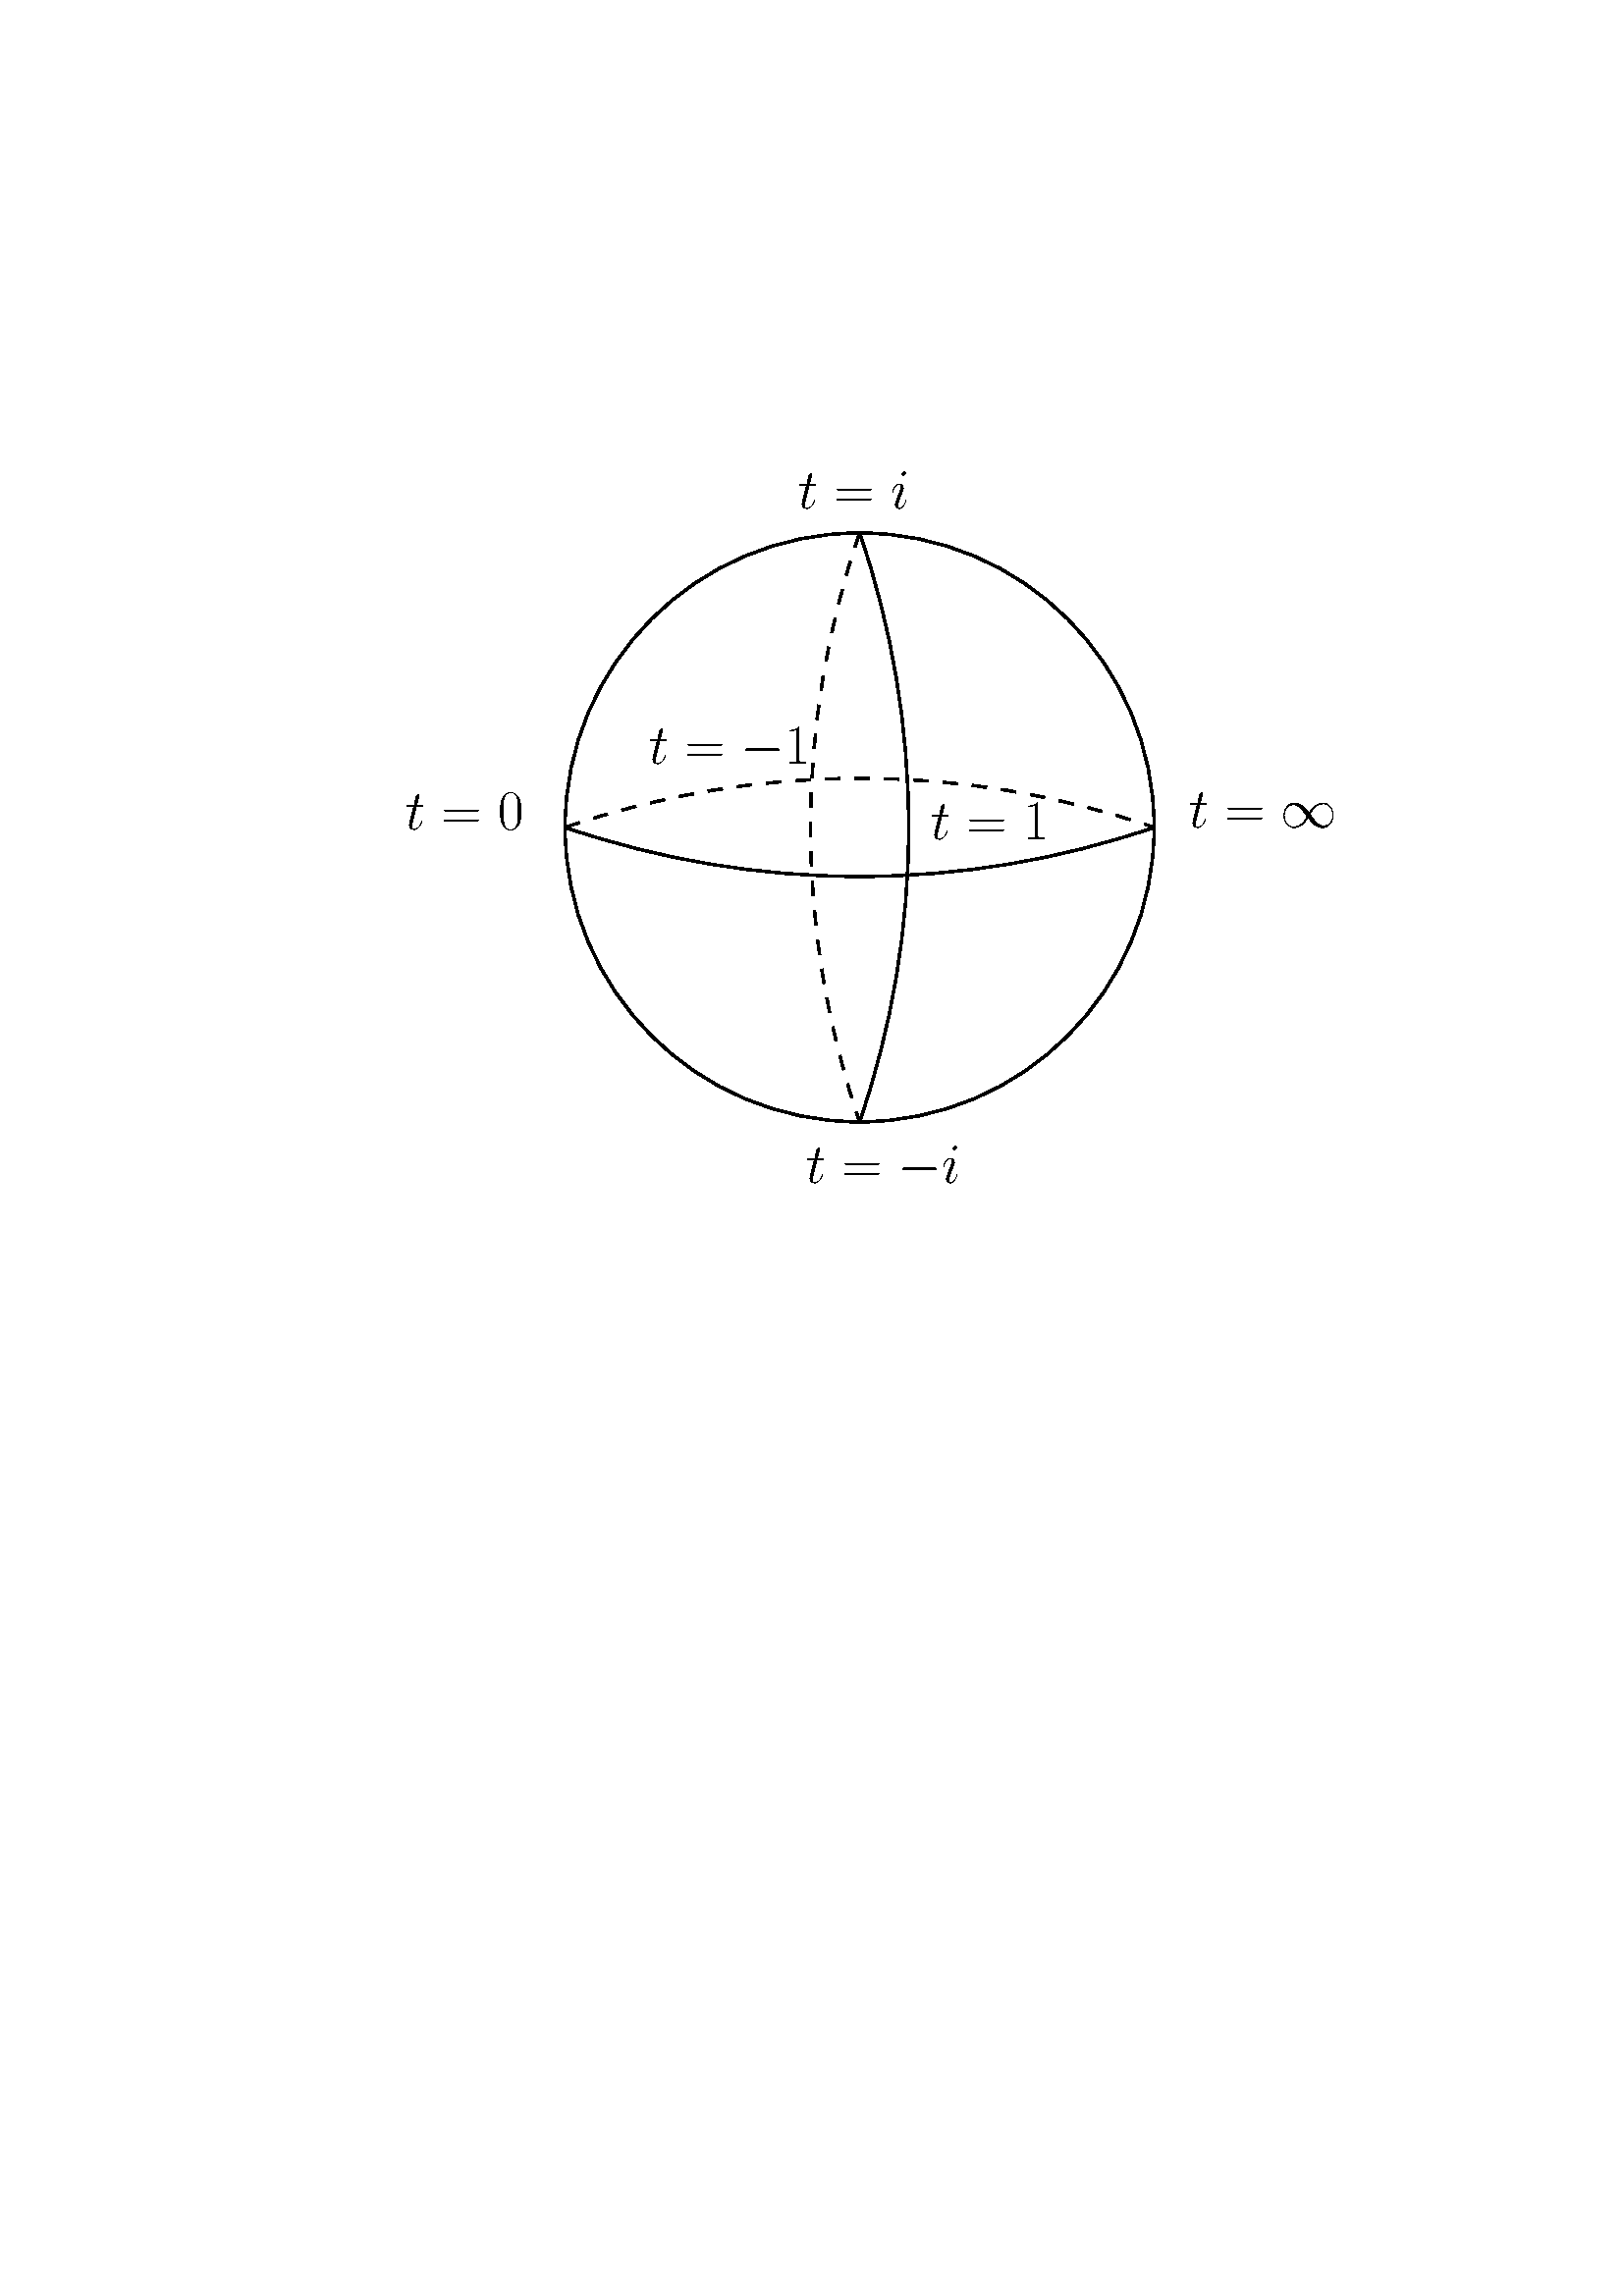
\includegraphics[width=0.75\linewidth]{figures/gla0-1.png}
\caption{ \medskip A family of topological field theories parametrized by the variable $t$.（原文 Fig.~1）}
\label{fig:zunko}
\end{figure}

The generators of $Spin'(4)$ are
$\Gamma_{\mu\nu}+\Gamma_{\mu+4,\nu+4}$, for $\mu,\nu=0,\dots,3$,
so a $Spin'(4)$-invariant spinor $\epsilon$ obeys
$(\Gamma_{\mu\nu}+\Gamma_{\mu+4,\nu+4})\epsilon=0$.  Setting
$\mu,\nu=0,1$, we learn that $\Gamma_{0145}\epsilon=\epsilon$, and
setting $\mu,\nu=2,3$, we learn that
$\Gamma_{2367}\epsilon=\epsilon$.  So
$\Gamma_0\Gamma_1\dots\Gamma_7\epsilon=\epsilon$, and using also
the chirality condition
$\Gamma_0\Gamma_1\dots\Gamma_9\epsilon=-i\epsilon$ of eqn.
\eqref{eq:nohinks}, we learn that
% 式 (3.11)
\setcounter{equation}{10}
\begin{equation}\label{eq:banother}
\Gamma_{89}\epsilon=-i\epsilon.
\end{equation}
 It follows in
particular that ${\cal K}=\Gamma_{89}$ acts with the same
eigenvalue $\EUK=-i{\cal K}=-1$ on $\epsilon_\ell $ and
$\epsilon_r$.  It also follows that $\Gamma_{8-i9}\epsilon=0$,
where $\Gamma_{8-i9}=(\Gamma_8-i\Gamma_9)/\sqrt 2$.  These facts
are helpful in verifying the supersymmetry transformation laws
presented below.

We now can see why this construction gives a family of topological
field theories parametrized by $\Bbb{CP}^1$ (\zunko).  We pick any
nonzero complex linear combination of $\epsilon_\ell$ and
$\epsilon_\rr$ % 式 (3.12)
\setcounter{equation}{11}
\begin{equation}\label{eq:utu}
\epsilon=u\epsilon_\ell+v\epsilon_\rr,
\end{equation}

and take this to be the generator of the topological symmetry.  An
overall scaling of $\epsilon$ would not matter, so the possible
choices for the topological symmetry are parametrized by
$\Bbb{CP}^1$. Because there is a natural choice of $\epsilon_\rr$
once $\epsilon_\ell$ is given, this has much more structure than
an abstract copy of $\Bbb{CP}^1$; it has a natural affine
parameter $t=v/u$.

We can use \eqref{eq:tokio}\ to determine the transformation of $u, v$, and
$t$ under $S$-duality.  Under an element $\gamma$ of the duality
group $\Gamma$, we have $\epsilon_\ell\to
\exp(i\hat\phi(\gamma))\epsilon_\ell$, $\epsilon_\rr\to
\exp(-i\hat\phi(\gamma))\epsilon_\rr$.  Hence, to ensure
invariance of $\epsilon=u\epsilon_\ell+v\epsilon_\rr$, we have
$u\to \exp(-i\hat\phi(\gamma))u$, $v\to \exp(i\hat\phi(\gamma))v$,
and finally the transformation of $t=v/u$ is % 式 (3.13)
\setcounter{equation}{12}
\begin{equation}\label{eq:duco}
t\to
\exp(2i\hat\phi(\gamma))t={{c\tau+d}\over\ {|c\tau+d|}}t.
\end{equation}

Similarly, we can determine the action on $t$ of the center of
$SU(4)_{{\cal R}}$. The generator ${\EUI}$ of the center acts by
$\epsilon_\ell\to i\epsilon_\ell$, $\epsilon_\rr\to
i^{-1}\epsilon_\rr$, so by a similar reasoning to the above, we
have % 式 (3.14)
\setcounter{equation}{13}
\begin{equation}\label{eq:ungu}
{\EUI}(t)=-t.
\end{equation}

Thus, the topological field theories with parameter $t$ or $-t$
are equivalent. This is a trivial equivalence in the sense that it
follows from a symmetry of the classical action -- as opposed to a
non-trivial $S$-duality.  The $\Bbb{Z}_2$ symmetry \eqref{eq:ungu}\ is the
only trivial equivalence among the twisted topological field
theories parametrized by $t$. In making this assertion, it is
essential that $\epsilon_\ell$ and $\epsilon_\rr$ have the same
eigenvalue of ${\cal K}$. Otherwise, a transformation in the group
$\Bbb{C}^*$ generated by ${\cal K}$ would act non-trivially on $t$
and would cause the whole $\Bbb{CP}^1$ family of topological field
theories to be trivially equivalent.  Of course, it is only
because there are (almost) no trivial equivalences that it is
possible for the non-trivial equivalences coming from $S$-duality
to generate something interesting like the geometric Langlands
program.

We write $Q_\ell$ and $Q_\rr$ for the supersymmetries generated by
$\epsilon_\ell$ and $\epsilon_\rr$. The supersymmetry generated by
the linear combination $\epsilon=u\epsilon_\ell+v\epsilon_\rr$ is
then % 式 (3.15)
\setcounter{equation}{14}
\begin{equation}\label{eq:hut}
Q=uQ_\ell+vQ_\rr,
\end{equation}
 and this is the topological
symmetry of the twisted theory. It is also convenient to write
% 式 (3.16)
\setcounter{equation}{15}
\begin{equation}\label{eq:nut}
\delta_T=\epsilon_\ell\delta_\ell+\epsilon_\rr\delta_\rr,
\end{equation}

where for any field $\Phi$,
% 式 (3.17)
\setcounter{equation}{16}
\begin{equation}\label{eq:but}
\delta_T\Phi=[Q,\Phi\},~~~\delta_\ell\Phi=
[Q_\ell,\Phi\},~~~\delta_\rr\Phi=[Q_\rr,\Phi\}.
\end{equation}
 ($T$  stands for
twisted or topological.)  Since $\epsilon_\ell$ and $\epsilon_r$
have $\EUK=-1$, it follows that $Q_\ell$, $Q_\rr$, and $Q$ all
have $\EUK=1$. Indeed, the supersymmetry transformation laws
presented below show explicitly that $\delta_T$ increases $\EUK$
by 1 for every field.  Thus in mathematical language, the space of
gauge-invariant operators or states is a complex, $\Bbb{Z}$-graded
by $\EUK$, with differential $Q$.

\par\medskip{\it The Fermion Fields And The Supersymmetry
Transformations}

The fermion fields $\lambda$ transform the same way as the
supersymmetry generators $\epsilon$, so using \eqref{eq:lollypop}\ and
\eqref{eq:tollypop}, we can identify them in four-dimensional terms. The
fields with ${\EUK}=1$ are two copies of $(\btwo,\btwo)^1$,
corresponding to two one-forms $\psi$ and $\tilde\psi$. The fields
transforming as $({\bf 3},{\bf 1})^{-1}$ and $(\bone,{\bf
3})^{-1}$ are the selfdual and anti-selfdual parts $\chi^\pm$ of a
two-form $\chi$ of ${\EUK}=-1$. Finally, there are two zero-forms
$\eta$ and $\tilde\eta$ of ${\EUK}=-1$.

It is helpful to define these four-dimensional fields more
precisely by specifying the following expansion of the
ten-dimensional spinor field $\lambda$ in terms of
four-dimensional fermion fields:\footnote{Since $\lambda$,
$\epsilon_\ell$, and $\epsilon_\rr$ are all of positive chirality,
this expansion must be made using only even elements of the
Clifford algebra. To ensure this, certain factors of
$\Gamma_{8+i9}={1\over \sqrt 2}\left(\Gamma_8+ i \Gamma_9\right)$
are included in the expansion.}
 % 式 (3.18)
\setcounter{equation}{17}
\begin{equation}\label{eq:iko}
\begin{aligned}\lambda=&\left(\eta
+\sum_\mu\Gamma^\mu\psi_\mu \Gamma_{8+i9}
+\sum_{\mu<\nu}\Gamma^{\mu\nu}\chi^+_{\mu\nu}\right)\epsilon_\ell
\\+& \left(\tilde\eta +\sum_{\mu}\Gamma^\mu\tilde\psi_\mu
\Gamma_{8+i9}+\sum_{
\mu<\nu}\Gamma^{\mu\nu}\chi^-_{\mu\nu}\right)\epsilon_\rr.\\\end{aligned}
\end{equation}

This formula uniquely determines sixteen fields ($\eta$ and
$\tilde\eta$, four components each of $\psi$ and $\tilde\psi$, and
six components of $\chi$) in terms of the sixteen components of
$\lambda$.  Note that, because
$\hat\Gamma_E\epsilon_\ell=-\epsilon_\ell$,
$\Gamma_{\mu\nu}\epsilon_\ell$ is selfdual, so
$\Gamma^{\mu\nu}\chi_{\mu\nu}\epsilon_\ell=\Gamma^{\mu\nu}\chi^+_{\mu\nu}\epsilon_\ell$.
Likewise
$\Gamma^{\mu\nu}\chi_{\mu\nu}\epsilon_\rr=\Gamma^{\mu\nu}\chi^-_{\mu\nu}\epsilon_\rr$.
So one could equivalently replace $\chi^\pm$ by $\chi$ in \eqref{eq:iko}.

It is convenient to normalize $\epsilon_\ell$ up to sign so that
% 式 (3.19)
\setcounter{equation}{18}
\begin{equation}\label{eq:zomop}
\bar\epsilon_\ell \Gamma_{8+i9}\epsilon_\ell = 1.
\end{equation}
 Then
it follows from $\epsilon_r=N\epsilon_\ell$ that likewise
% 式 (3.20)
\setcounter{equation}{19}
\begin{equation}\label{eq:omop}
\bar\epsilon_r\Gamma_{8+i9}\epsilon_r=1.
\end{equation}
 {}From
considerations of four-dimensional chirality, it follows that
% 式 (3.21)
\setcounter{equation}{20}
\begin{equation}\label{eq:tomop}
\bar\epsilon_\ell\Gamma_{8+i9}\epsilon_r
=\bar\epsilon_r\Gamma_{8+i9}\epsilon_\ell=0.
\end{equation}

The next step is to describe how the fields transform under the
topological symmetries, that is, the supersymmetries generated by
$\epsilon_\ell$ and $\epsilon_\rr$.   For example, to transform
the bosons, we start with $\delta_S A_I=i\bar\epsilon
\Gamma_I\lambda$. Upon setting $\epsilon =
u\epsilon_\ell+v\epsilon_\rr$, we get for the four-dimensional
gauge field % 式 (3.22)
\setcounter{equation}{21}
\begin{equation}\label{eq:kono}
\delta_T A_\mu = iu\bar \epsilon_\ell
\Gamma_\mu \lambda +iv\bar\epsilon_\rr\Gamma_\mu\lambda.
\end{equation}
 After
some $\Gamma$-matrix gymnastics, one finds the transformation of
the four-dimensional gauge field under the topological
supersymmetry: % 式 (3.23)
\setcounter{equation}{22}
\begin{equation}\label{eq:bono}
\delta_T A_\mu=iu
\psi_\mu+iv\tilde\psi_\mu.
\end{equation}
 Similarly, for the other bosonic
fields we find % 式 (3.24)
\setcounter{equation}{23}
\begin{equation}\label{eq:lono}
\delta_T\phi_\mu=iv\psi_\mu -
iu\tilde\psi_\mu.
\end{equation}
 % 式 (3.25)
\setcounter{equation}{24}
\begin{equation}\label{eq:otono}
\begin{aligned}\delta_T\sigma & = 0 \\
                       \delta_T\bar\sigma & = iu\eta+iv\tilde\eta.\\\end{aligned}
\end{equation}

The vanishing of $\delta_T\sigma$ actually follows merely from the
fact that $\sigma$ has ${\EUK}=2$, and there is no appropriate
field of ${\EUK}=3$.

Likewise, we can find the transformations of the four-dimensional
fermionic fields starting with the underlying transformation law
% 式 (3.26)
\setcounter{equation}{25}
\begin{equation}\label{eq:invo}
\delta_T\lambda=\half\sum_{I,J=0}^9F_{IJ}\Gamma^{IJ}\epsilon,
\end{equation}

where $\epsilon=u\epsilon_\ell+v\epsilon_\rr$. The fermionic
fields with ${\EUK}=-1$ transform by
% 式 (3.27)
\setcounter{equation}{26}
\begin{equation}\label{eq:helpme}
\begin{aligned}\delta_T\chi^+ & = u(F-\phi\wedge\phi)^+
+v(D\phi)^+\\ \delta_T\chi^-& = v(F-\phi\wedge\phi)^- -
u(D\phi)^-\\ \delta_T\eta& = vD^*\phi+u[\bar\sigma,\sigma] \\
\delta_T\tilde\eta& = -uD^* \phi+v[\bar\sigma,\sigma].\\\end{aligned}
\end{equation}
 Those
of ${\EUK}=1$ transform by % 式 (3.28)
\setcounter{equation}{27}
\begin{equation}\label{eq:mimo}
\begin{aligned}\delta_T\psi& = u\,
D\sigma +v[\phi,\sigma]\\ \delta_T\tilde\psi & = v\, D\sigma - u
[\phi,\sigma].\\\end{aligned}
\end{equation}
 In these formulas, $D=d+[A,\,\cdot \,]$ is the
covariant derivative with respect to the connection $A$; a Lie
bracket is implicit in the adjoint-valued two-form
$\phi\wedge\phi$; and $D^*\phi=\star D \star \phi =
D_\mu\phi^\mu$, with $\star$ the Hodge star.
